\chapter{Sistema de seguimiento}

Un sistema de seguimiento se puede dividir en tres etapas bien definidas:
\begin{enumerate}
 \item Entrenamiento
 \item Detección
 \item Seguimiento cuadro a cuadro
\end{enumerate}

La etapa de entrenamiento consiste en obtener una representación del objeto al cuál se pretende seguir. Para llevarla a cabo se puede utilizar un patrón (template) ya conocido o aprenderlo de imágenes capturadas del mismo objeto. Luego se utiliza en la detección para ubicar la representación del objeto dentro de una imagen cualquiera. Una vez conocido el template no se requiere de una nueva ejecución del entrenamiento.

La segunda etapa, la de detección, radica en encontrar dentro de un frame del video al objeto en cuestión utilizando el método de detección deseado, valiéndose de la información obtenida en la etapa de entrenamiento. Esta etapa se ejecuta, con el propósito de encontrar en la imagen el objeto a seguir, al comienzo del sistema de seguimiento y cuando el seguimiento cuadro a cuadro falla. Dado que la etapa de detección suele ser la más costosa en términos de desempeño computacional es deseable que se ejecute la menor cantidad de veces posible.

Finalmente, la tercera etapa consiste en seguir cuadro a cuadro el objeto detectado en la etapa anterior. Es decir, teniendo la ubicación del objeto en un cuadro de video se desea identificar la posición del mismo objeto en el siguiente frame. Esta etapa es la más importante ya que es la que se ejecuta en cada frame del video. La eficiencia del método de seguimiento es lo que determinará que todo el sistema de seguimiento se consiga realizar eficientemente. Si la técnica de seguimiento tiene una efectividad baja, es decir, no logra identificar la nueva posición del objeto en el siguiente cuadro, se debe volver a la etapa de detección cuyo desempeño computacional es mayor.

Tomando como base estas etapas, proponemos distintos métodos para cada una de ellas tanto para RGB como para D y RGB-D. La primera etapa del sistema puede ser prescindible si contamos con el modelo RGB-D del objeto a seguir y una cámara calibrada. Este es el caso de estudio de esta tesis, ya que, con el propósito de poder evaluar cuantitativamente el seguimiento de objetos en secuencias de imágenes RGB-D, utilizamos la base de datos descripta en la sección \ref{base_rgbd}.

\section{Método propuesto RGB}\label{metodo_rgb}
\subsection{Entrenamiento}
\subsection{Detección}
\subsection{Seguimiento}

\section{Método propuesto en D}
\subsection{Alignment prerejective}\label{alignment_prerejective}

\subsection{Iterative Closest Point (ICP)}

Para esta primera etapa existen varias posibilidades distintas que van desde utilizar una única nube de puntos hasta generar un modelo completo del objeto 3D alineando todas las nubes de puntos disponibles en la base. \comentarioM{La tarea de generar un modelo completo excede el tema de estudio de esta tesis. Además el modelo resultante se utilizara únicamente para la etapa de detección por lo que se optó por el método más simple que es tomar una nube de puntos cualquiera del objeto a seguir como modelo 3D.}\comentarioP{Quedó afuera porque nos enfocamos en tracking} Por estos motivos se decidió elegir una nube de puntos fija para cada objeto, en particular, la que posee rotación 0. Otra posibilidad es elegir de todas las nubes de puntos de cada objeto presentes en la base alguna cualquiera al azar. Esto resulta más realista pero sería un problema al momento de analizar los resultados ya que se agregaría una variante azarosa y se deberían correr muchas veces la misma prueba para lograr un análisis más acertado.


\begin{figure}
	\centering
	\begin{subfigure}[b]{0.25\textwidth}
		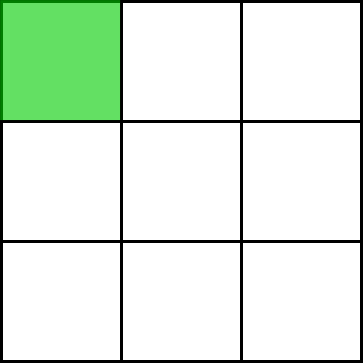
\includegraphics[width=\textwidth]{img/primercuadrante.png}
		\caption{Primer frame de búsqueda}
		\label{frames_solapados_1}
	\end{subfigure}
	\quad
	\begin{subfigure}[b]{0.25\textwidth}
		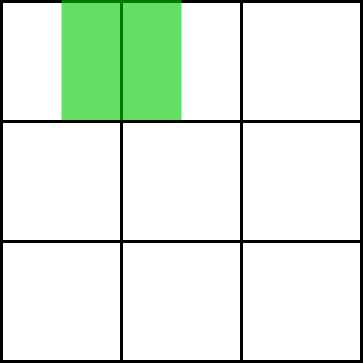
\includegraphics[width=\textwidth]{img/segundocuadrante.png}
		\caption{Segundo frame de búsqueda}
		\label{frames_solapados_2}
	\end{subfigure}	
	\quad
	\begin{subfigure}[b]{0.25\textwidth}
		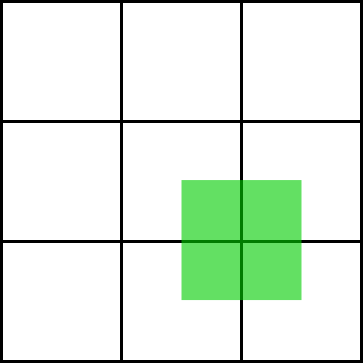
\includegraphics[width=\textwidth]{img/decimonovenocuadrante.png}
		\caption{$19^{\circ}$ frame de búsqueda}
		\label{frames_solapados_3}
	\end{subfigure}
	\caption{Se busca en cada cuadrante de la grilla y en los recuadros del mismo tamaño que cubren los bordes de la grilla principal}
	\label{frames_solapados}
\end{figure}

Para la segunda etapa, la de detección, se utilizó el método descripto en la sección \ref{alignment_prerejective} refinando el resultado con ICP. La elección del mismo se realizó luego de correr varias pruebas que corroboraran la factibilidad del mismo. En estas pruebas también se observó que si la región donde se buscaba el objeto era lo suficientemente pequeña la búsqueda era más robusta.\comentarioP{Mejor más chica?} Teniendo en cuenta esto se pensó en una variante para la detección que utilice el método elegido. Esta tiene como primer paso obtener el alto y el ancho del modelo del objeto a seguir y escalarlos según un valor, llamado \param{detection\_frame\_size}. Considerando estos valores dividimos la escena en cuadrantes de ese tamaño y corrimos el método de detección en cada cuadrante. Con el fin de detectar el objeto cuando el mismo se extiende sobre dos o más regiones, la búsqueda se hizo utilizando un marco que recorre todos los cuadrantes y sus uniones, como puede observarse en el gráfico \ref{frames_solapados}. Notar que la división por cuadrantes solo se realizó en los ejes ``x'' e ``y'' y no en el eje de profundidad ya que las pruebas preeliminares dieron buenos resultados de esta manera y hacer eso implicaba agregarle complejidad algoritmica al método. La detección se corre en cada uno de estos cuadrantes y pueden suceder varias cosas:
\begin{itemize}
	\item No se encontró el objeto en ningún cuadrante: en este caso el algoritmo indica que el objeto no se encuentra en el frame
	\item Se encontró el objeto en un cuadrante
	\item Se encontró el objeto en varios cuadrantes: el algoritmo devuelve la mejor posición encontrada según un puntaje de buena alineación devuelto por el algoritmo \ap.
\end{itemize}

Si la detección es positiva, se refina la alineación corriendo ICP entre el modelo del objeto transformado por el método ``alignment prerejective'' y el cuadrante de la escena donde fue encontrado el mismo. Con el objetivo de comenzar el seguimiento en las mejores condiciones posibles, se intentan tomar los puntos del objeto buscado pertenecientes a la escena. Esto se realiza porque se asume que el objeto se va modificando cuadro a cuadro, ya sea por movimientos de la cámara o del objeto. Una de las formas para obtener los puntos del modelo del objeto en la escena es utilizando un \kdt\footnote{AGREGAR REFERENCIA A KDTREE}. \comentarioP{Explicar un poco que es un kdtree} Se arma un \kdt con los puntos provenientes del modelo alineado y se filtran uno a uno los puntos de la escena que se encuentren cerca de al menos un punto del modelo en un cierto radio de distancia. Este valor de radio es uno de los parámetros explorados durante las pruebas, llamado \param{leaf\_size}. Los puntos que surjan de esta búsqueda son los considerados encontrados en la escena. Para que el algoritmo de búsqueda considere exitosa la detección, la cantidad de puntos filtrados de la escena debe ser mayor o igual al 50\% de los puntos del modelo original. Si todas estas etapas son superadas con éxito, se considera que el objeto fue encontrado y se pasa a la siguiente etapa de seguimiento. Si cualquiera de estos pasos fallara, se comienza nuevamente con la etapa de detección en el siguiente frame.

La tercera y última etapa BLABLABLA

\subsection{Entrenamiento}

\subsection{Detección}


\subsection{Seguimiento}

\section{Método propuesto en RGB-D}

\subsection{Entrenamiento}

\subsection{Detección}

\subsection{Seguimiento}










\chapter{Base de datos RGB-D}\label{base_rgbd}
Durante el desarrollo de este trabajo se utilizaron secuencias con información de ground truth de imágenes RGB-D anotadas para aplicar los métodos estudiados y tener una referencia para hacer comparaciones y sacar conclusiones sobre su eficacia. Las escenas fueron tomados del trabajo \cite{lai2011large} en donde se creó una base de objetos y escenas. Esta base cuenta con varias escenas. Cada una de ellas consta de varios frames RGB con su respectiva información de profundidad. Además, la base provee información frame a frame de qué objetos aparecen y cuál es su ubicación en el plano RGB.

{\huge Figura con ejemplos de las escenas, por ejemplo: 2 filas con varias columnas cada una en donde haya frames RGB arriba y sus equivalentes en depth abajo}

Por otra parte, la base provee imágenes RGB-D de los objetos presentes en las escenas antes mencionadas con el objetivo de obtener su representación 3D.\comentarioP{Comentar como fueron adquiridas la resolución, longitud y ¿?} Cada una de estas imágenes es acompañada además por una máscara que segmenta al objeto buscado y la información de profundidad (nube de puntos) del objeto segmentado. Para tomar estas imágenes los objetos fueron posados en una base circular giratoria y manteniendo la cámara en una posición fija se tomaron muestras con cierta regularidad cubriendo toda la circunferencia de cada objeto. Esto se hizo además desde distintas alturas permitiendo apreciar la profundidad del objeto y así obtener una mejor descripción del mismo.

Los objetos elegidos para esta base se organizaron de una manera jerárquica tomada de las relaciones hiperónimo/hipónimo de WordNet. Cada objeto pertenece a una clase de objetos y hay varias instancias por cada clase. Por ejemplo, en la categoría ``taza'' existen varias instancias diferentes, que se corresponden simplemente a distintas tazas ya sea por forma o por color.\comentarioM{No hice pruebas usando varias instancias de un mismo objeto...}

Existen distintas escenas que contienen a los objetos mencionados y en cada escena se combinan distintas clases de objetos y distintas instancias de la misma clase. De esta manera la base otorga la posibilidad de verificar algoritmos capaces de identificar instancias de objetos particulares o familias de objetos según la clasificación antes mencionada.






\section{Parte de la propuesta que quedó afuera}



La detección se realizó utilizando \cite{6630856} y corrigiendo con ICP.
Cosas a escribir:
\begin{itemize}
	\item qué sucedió al tratar de detectar en toda la escena
	\item cómo se hizo para dividir la escena en partes y detectar en cada una
\end{itemize}


La utilización del algoritmo ICP \cite{zhang94icp,besl92icp} para realizar el seguimiento resulta natural e intuitiva. Por ello, es que en esta tesis se estudiará el algoritmo ICP y sus variantes \cite{estepar2004robust,segal2009generalized}, con el fin de evaluar cómo sus parámetros afectan cuantitativamente al sistema de seguimiento y la performance computacional del mismo. Asimismo, se evaluará la adaptabilidad del filtro de Kalman \cite{welch1995introduction} para seguimiento de objetos 3D en imágenes RGB-D con posibilidad de desempeño en tiempo real. El filtro de Kalman es un filtro muy popular y estudiado extensivamente en la literatura \cite{julier1997new,wan2000unscented} debido a su gran desempeño para realizar seguimiento en imágenes 2D. Por lo tanto, su aplicación en seguimiento de objetos 3D resulta de especial interés.

\section{Elección de parámetros}\label{eleccion_parametros}

\begin{table}[h]
\scriptsize
    \begin{tabular}{|l|*{3}{c|}*{3}{c|}*{3}{c|}}
        \hline 
    Método & \multicolumn{3}{|c|}{coffee\_mug\_5} & \multicolumn{3}{|c|}{cap\_4} & \multicolumn{3}{|c|}{bowl\_3}\\
    \hline 
                         & \% Over. & STD & \% foll. & \% Over. & STD & \% foll. & \% Over. & STD & \% foll. \\
    \hline
    \textbf{Bhatta. ch. verde} & 38.52 & 32.50 & 85.53 & 54.37 & 18.52 & 87.80 & 64.95 & 43.44 & 40.00\\
    \hline
    Correl. ch. verde          & 21.68 & 31.54 & 90.79 & 49.88 & 11.07 & 97.56 & 46.84 & 44.30 & 60.91\\
    \hline
    Bhatta. x canal            & 33.76 & 20.11 & 94.74 & 49.95 & 14.01 & 95.12 & 10.96 & 22.78 & 97.27\\
    \hline
    RGB y HSV                  & 39.32 & 25.19 & 92.11 & 56.69 & 21.39 & 82.93 & 73.32 & 40.70 & 30.91\\
    \hline
    \end{tabular}
\caption{Corregir valores!}
\end{table}